\chapter{Asymmetric Radial Gradient Echoes}
\chaptermark{Asymmetric Radial Gradient Echoes} \label{Chp:asym-echo}

Asymmetric-echo radial sampling is an interesting sampling scheme because it shortens the echo time and thus reduces off-resonance effects. In contrast to the k-space line (echo)-reduction undersampling scheme, it samples an incomplete echo, which poses a different reconstruction problem on how to estimate the missing portion of the echo. Therefore, this chapter studies the characteristics of asymmetric radial gradient echoes and associated image reconstruction methods. Moreover, the application of this sampling scheme to real-time phase-contrast flow MRI is investigated. Here, asymmetric echoes allow for the integration of motion-compensation gradients while maintaining or even improving temporal resolution. Consequently, flow MRI with motion compensation and short \acs{TE} reduces signal loss due to intra-voxel phase dispersion and turbulence \cite{2015_PC_rev}.

\section{Undersampled Radial FLASH with Asymmetric Echoes}
For asymmetric echo data sampling, also known as partial echo in partial Fourier imaging \cite{2004_MRI_Bernstein}, every k-space readout line is only partially collected before reaching the center of k-space. This is achieved by reducing the moment of the corresponding pre-dephasing gradient, as shown in the sequence diagram (left part of \cref{Fig:aysm-echo-seq-ksp}). Therefore, it shortens the readout gradient before the echo center and reduces the TE and TR, while the readout period after the echo center remains the same as for symmetric echo. Here, an asymmetry metric (in $\%$) is quantified as $100 \times A / (2 B)$ with $A$ and $B$ the durations of the acquisition window before and after the echo center, respectively. With this definition, \SI{50}{\percent} asymmetry corresponds to a symmetric echo, while \SI{0}{\percent} represents a half-echo acquisition. The k-space trajectory depicted in the right part of \cref{Fig:aysm-echo-seq-ksp} demonstrates the extreme azimuthal undersampling with only seven spokes per image and \SI{20}{\percent} asymmetry.

As has been demonstrated in \cite{2004_MRI_Bernstein}, the first row of \cref{Fig:aysm-echo-psf} shows that the artifact-free area of the simulated point spread functions (\acsp{PSF}) reconstructed via direct Gridding \& FFT decreases along the number of symmetric spokes acquired, but the central lobe is not distorted or folded-in as is commonly seen in undersampled Cartesian sampling. Furthermore, the streaks are much better spatially resolved and more severe with less number of spokes. On the other hand, when the number of spokes is kept at \num{125} and the asymmetry is reduced from \SI{40}{\percent} to \SI{30}{\percent} and \SI{20}{\percent} (see the second row of \cref{Fig:aysm-echo-psf}), a bright ring surrounding the central white lobe emerges and eventually reduces the artifact-free area. This may result in blurring and Gibbs ringing artifacts due to the lack of high spatial-frequency data. 
\begin{figure}[p]
  \centering
  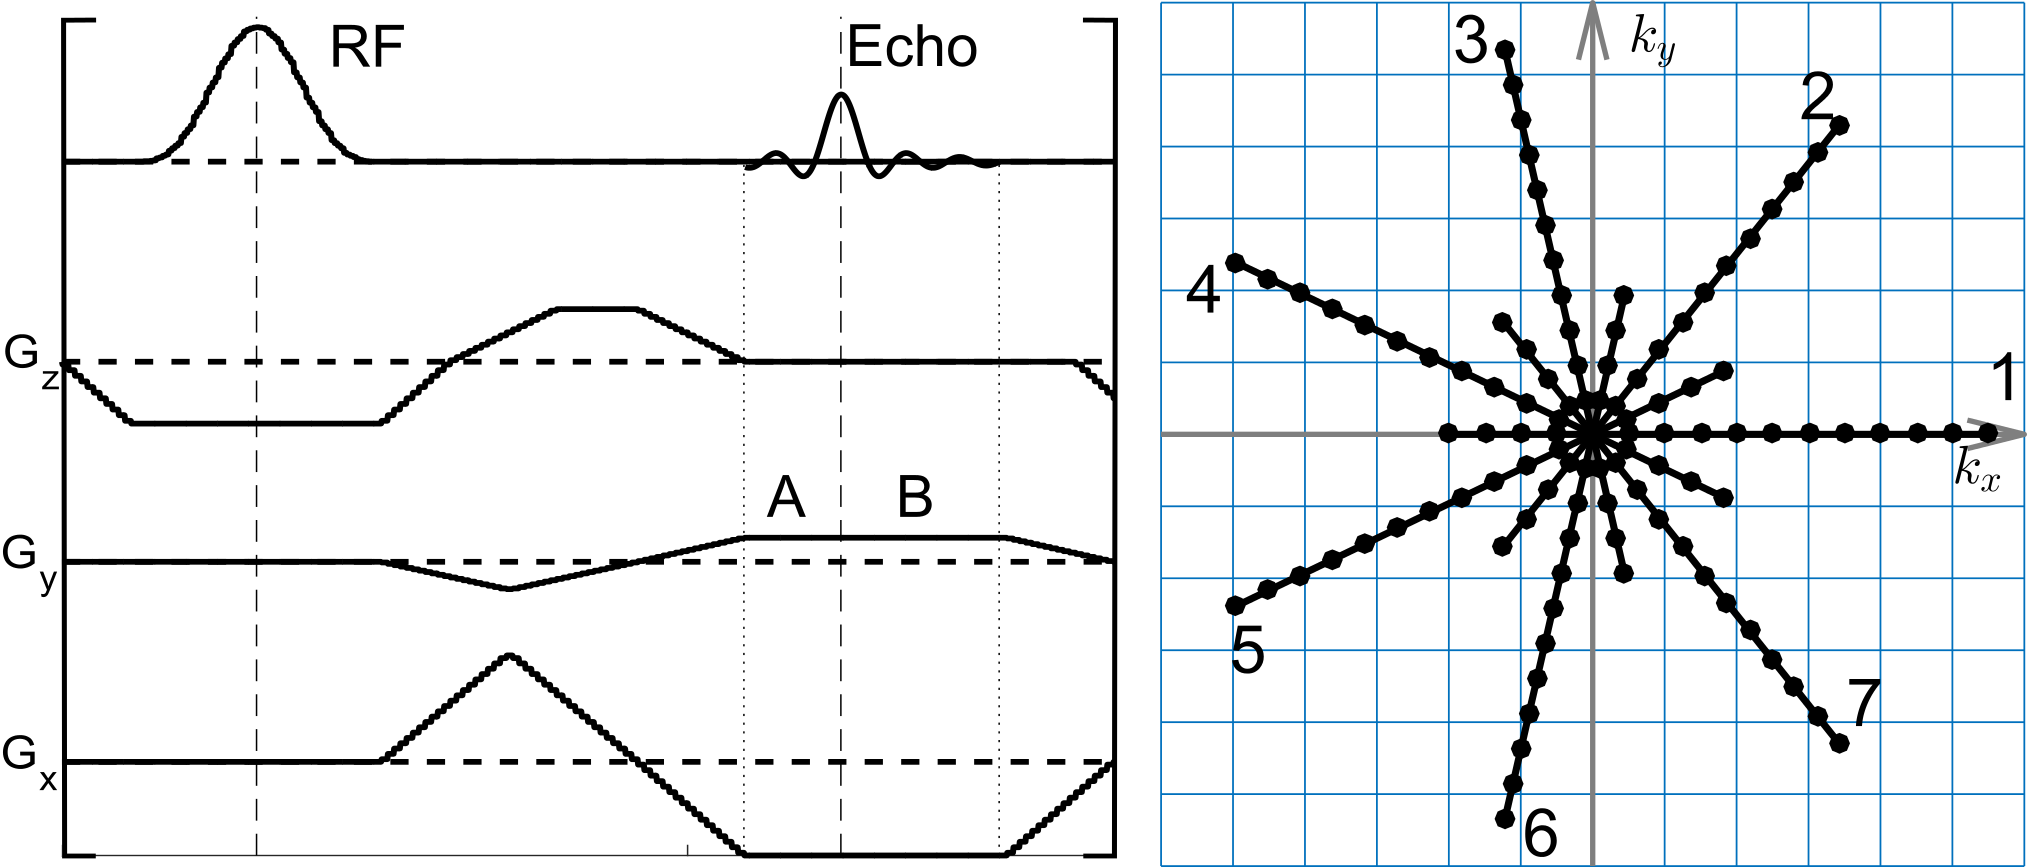
\includegraphics[width=0.85\textwidth]{fig/asym-echo-seq-ksp.png}
  \caption{Real-time radial FLASH with asymmetric gradient echoes. Left: The sequence diagram represents one repetition cycle for the acquisition of one asymmetric echo. Right: Corresponding k-space trajectory with seven spokes with \SI{20}{\percent} asymmetry and $2\pi$ radial angle coverage. The blue lines represent a 2D Cartesian grid. } \label{Fig:aysm-echo-seq-ksp}
  
  \par\bigskip
  
  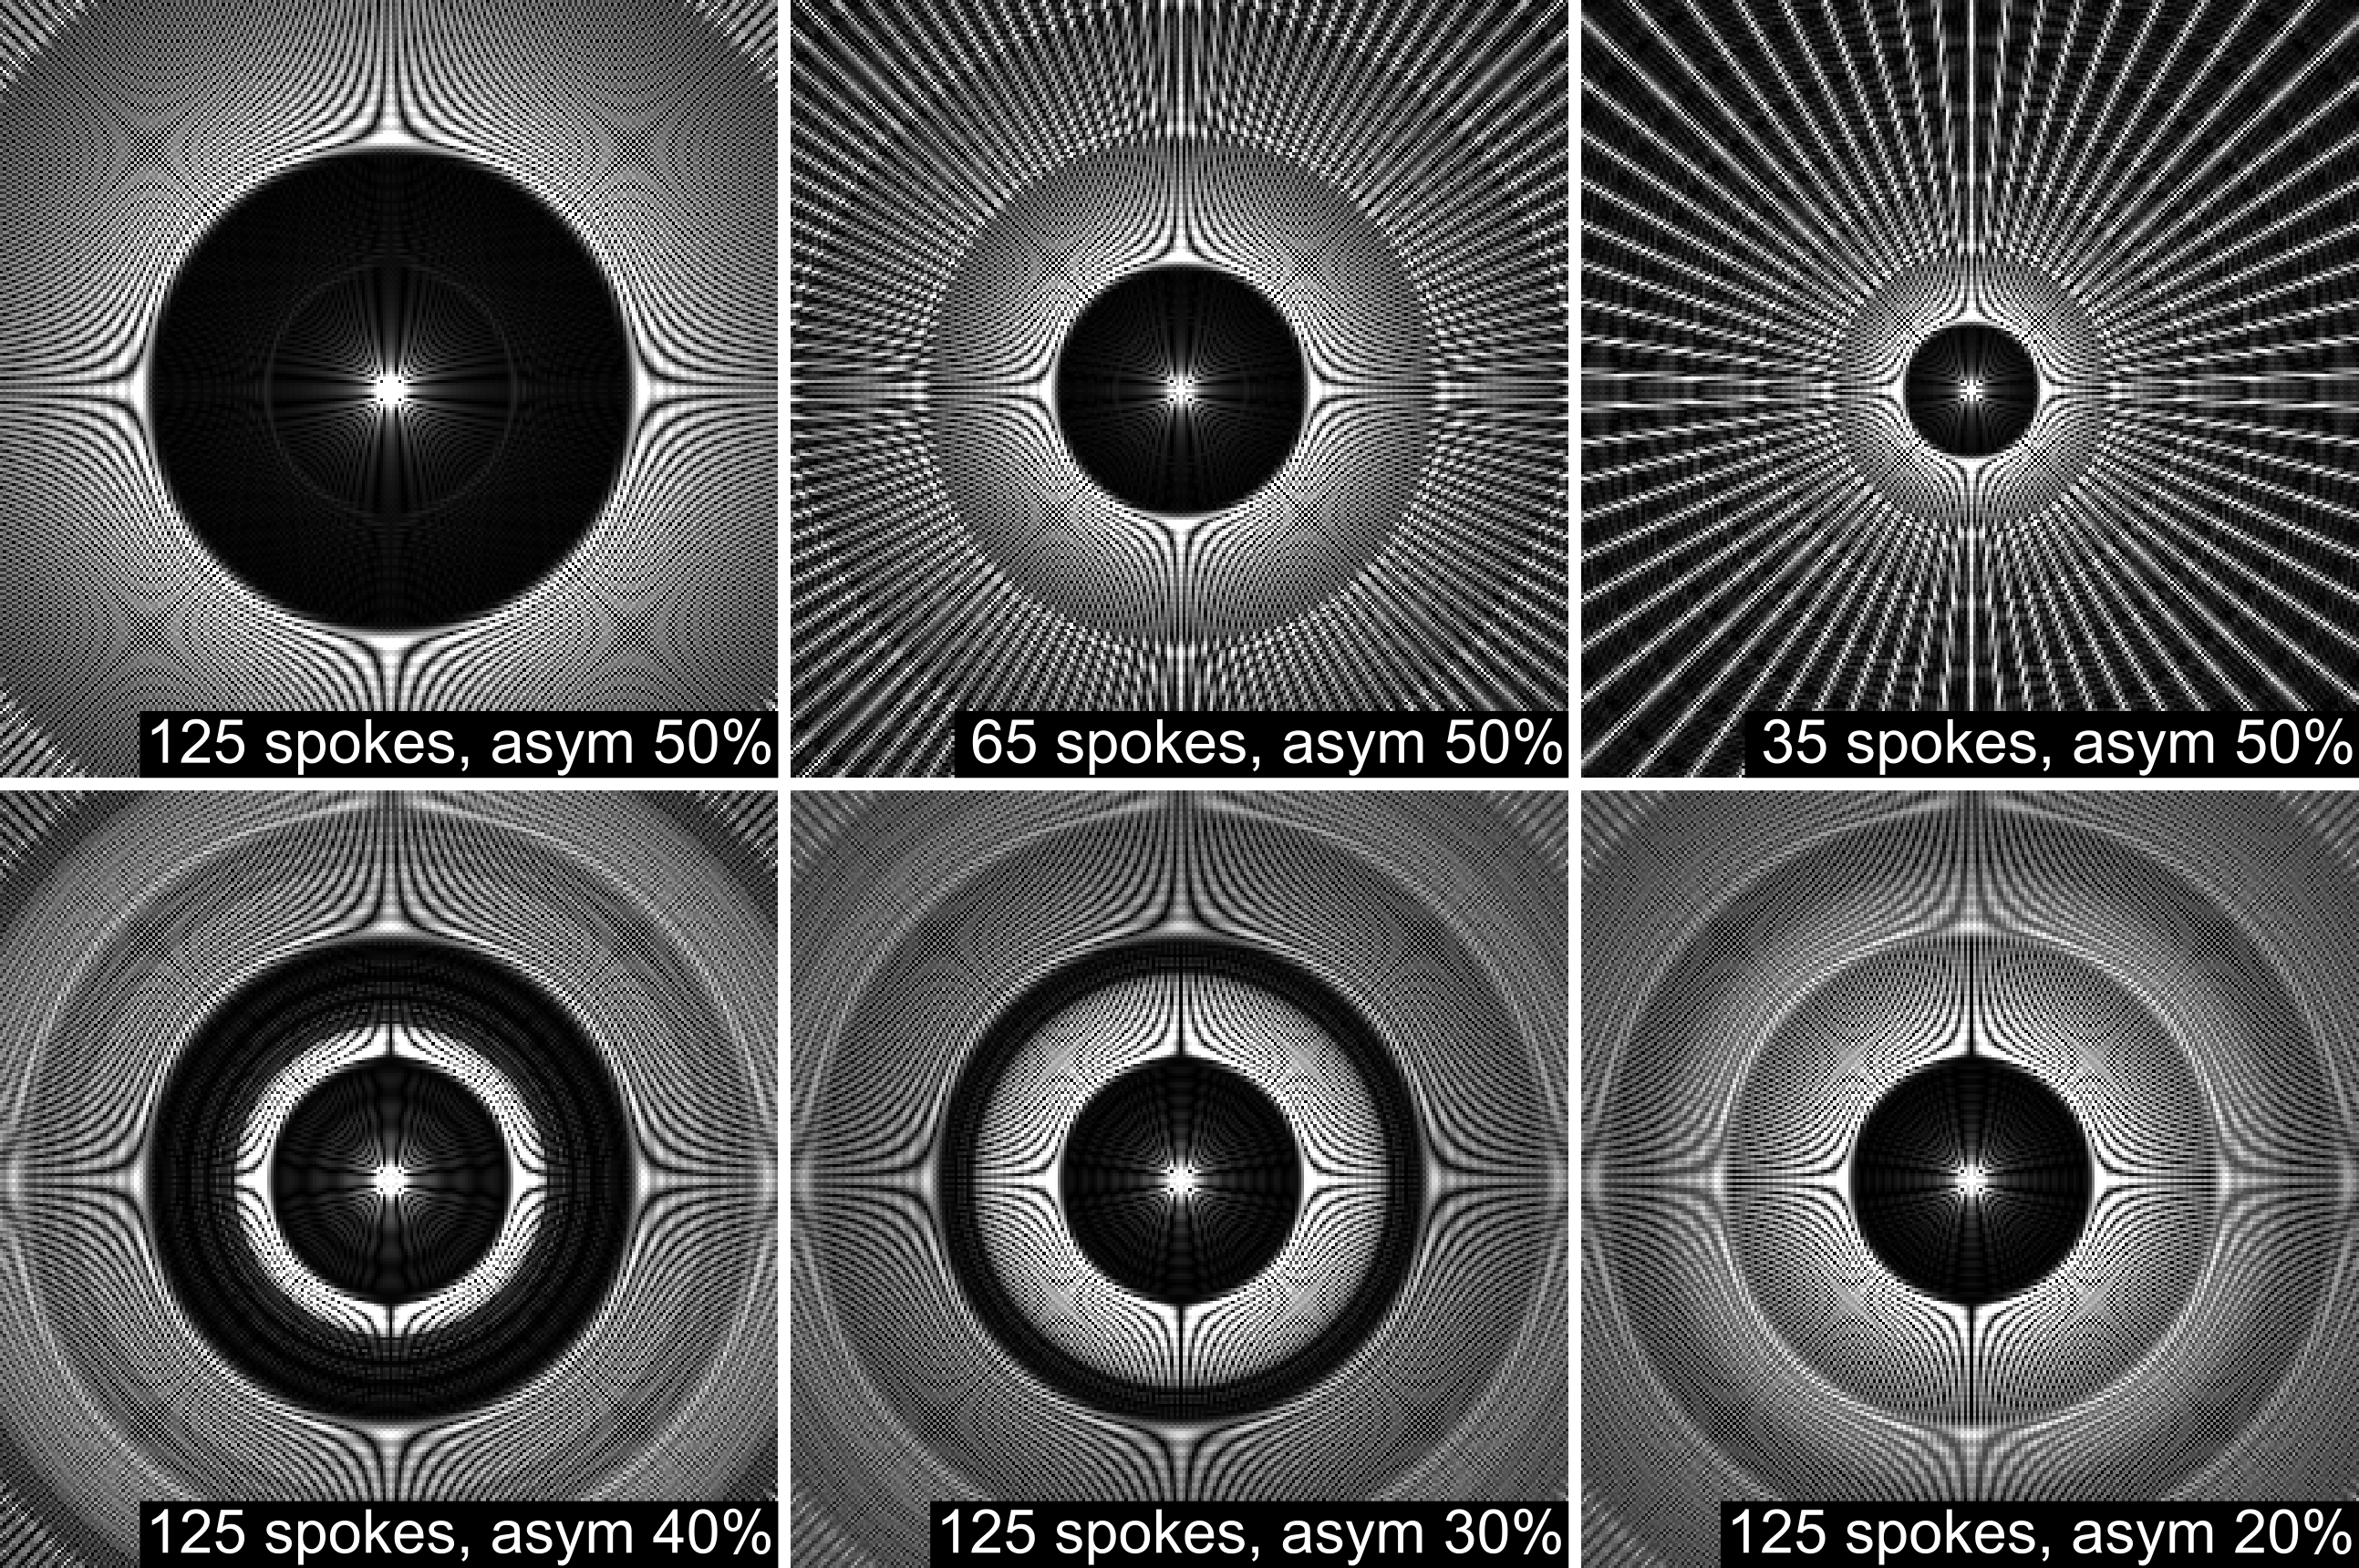
\includegraphics[width=0.85\textwidth]{fig/asym-echo-psf.png}
  \caption{Simulated \acsp{PSF} via Gridding \& FFT reconstruction with $2\pi$ radial angle coverage, 256 total readout samples. The \acs{PSF} in the first row was acquired with (left) \num{125}, (center) \num{65}, and (right) \num{35} symmetric spokes, while the second row was acquired with 125 spokes and (left) \SI{40}{\percent}, (center) \SI{30}{\percent}, and (right) \SI{20}{\percent} asymmetry. The central white lobe of the \acsp{PSF} indicates the reconstructed point. The artifact-free area is the solid black region around the central lobe.} \label{Fig:aysm-echo-psf}
\end{figure}

Another appealing feature of asymmetric echo is that it keeps the same spatial resolution as symmetric echo. It is well known that the spatial resolution is inversely proportional to the maximum gradient areas in two readout directions, which are equivalent to $k_{x,\text{max}}$ and $k_{y,\text{max}}$, respectively \cite{2010_principle_mri}. As the radially-supported FOV in k-space for asymmetric echo is the same as that for symmetric echo, the spatial resolution retains for asymmetric-echo sampling. As shown in \cref{Fig:aysm-echo-spatialRes}, where simulated asymmetric k-space data was generated from a symmetric measurement (i.e.~\SI{50}{\percent} asymmetry) for a standard multi-purpose phantom of the vendor. Respective FLASH acquisition parameters were: TR/TE = \num{2.48}/\SI{1.62}{\ms}, flip angle \ang{8}, \SI{212}{\mm} FOV, \SI{0.83}{\mm} in-plane resolution, \SI{8}{\mm} slice thickness, \num{15} spokes and \num{5} sequential-interleaving turns. Simulated gradient-echo data with \SI{40}{\percent}, \SI{30}{\percent}, and \SI{20}{\percent} asymmetry were obtained by cropping a respective number of data samples from the leading parts of corresponding symmetric spokes. True asymmetric measurements of the resolution phantom for \SI{40}{\percent}, \SI{30}{\percent}, and \SI{20}{\percent} asymmetry used similar experimental parameters as the symmetric measurement except for the shortest possible repetition and echo times: TR/TE (\SI{40}{\percent}) = \num{2.31}/\SI{1.45}{\ms}, TR/TE (\SI{30}{\percent}) = \num{2.14}/\SI{1.28}{\ms}, and TR/TE (\SI{20}{\percent}) = \num{1.99}/\SI{1.13}{\ms}. The spatial resolution of all images in \cref{Fig:aysm-echo-spatialRes} is well maintained, although increasing asymmetry leads to fewer samples in the outer (e.g.~high spatial frequency) regions of k-space. This is clearly demonstrated by the well-resolved first three rows of water-filled holes in \cref{Fig:aysm-echo-spatialRes} with diameters ranging from \SI{2.5}{\mm} to \SI{2.0}{\mm} and \SI{1.5}{\mm}.
\begin{figure}[tb]
  \centering
  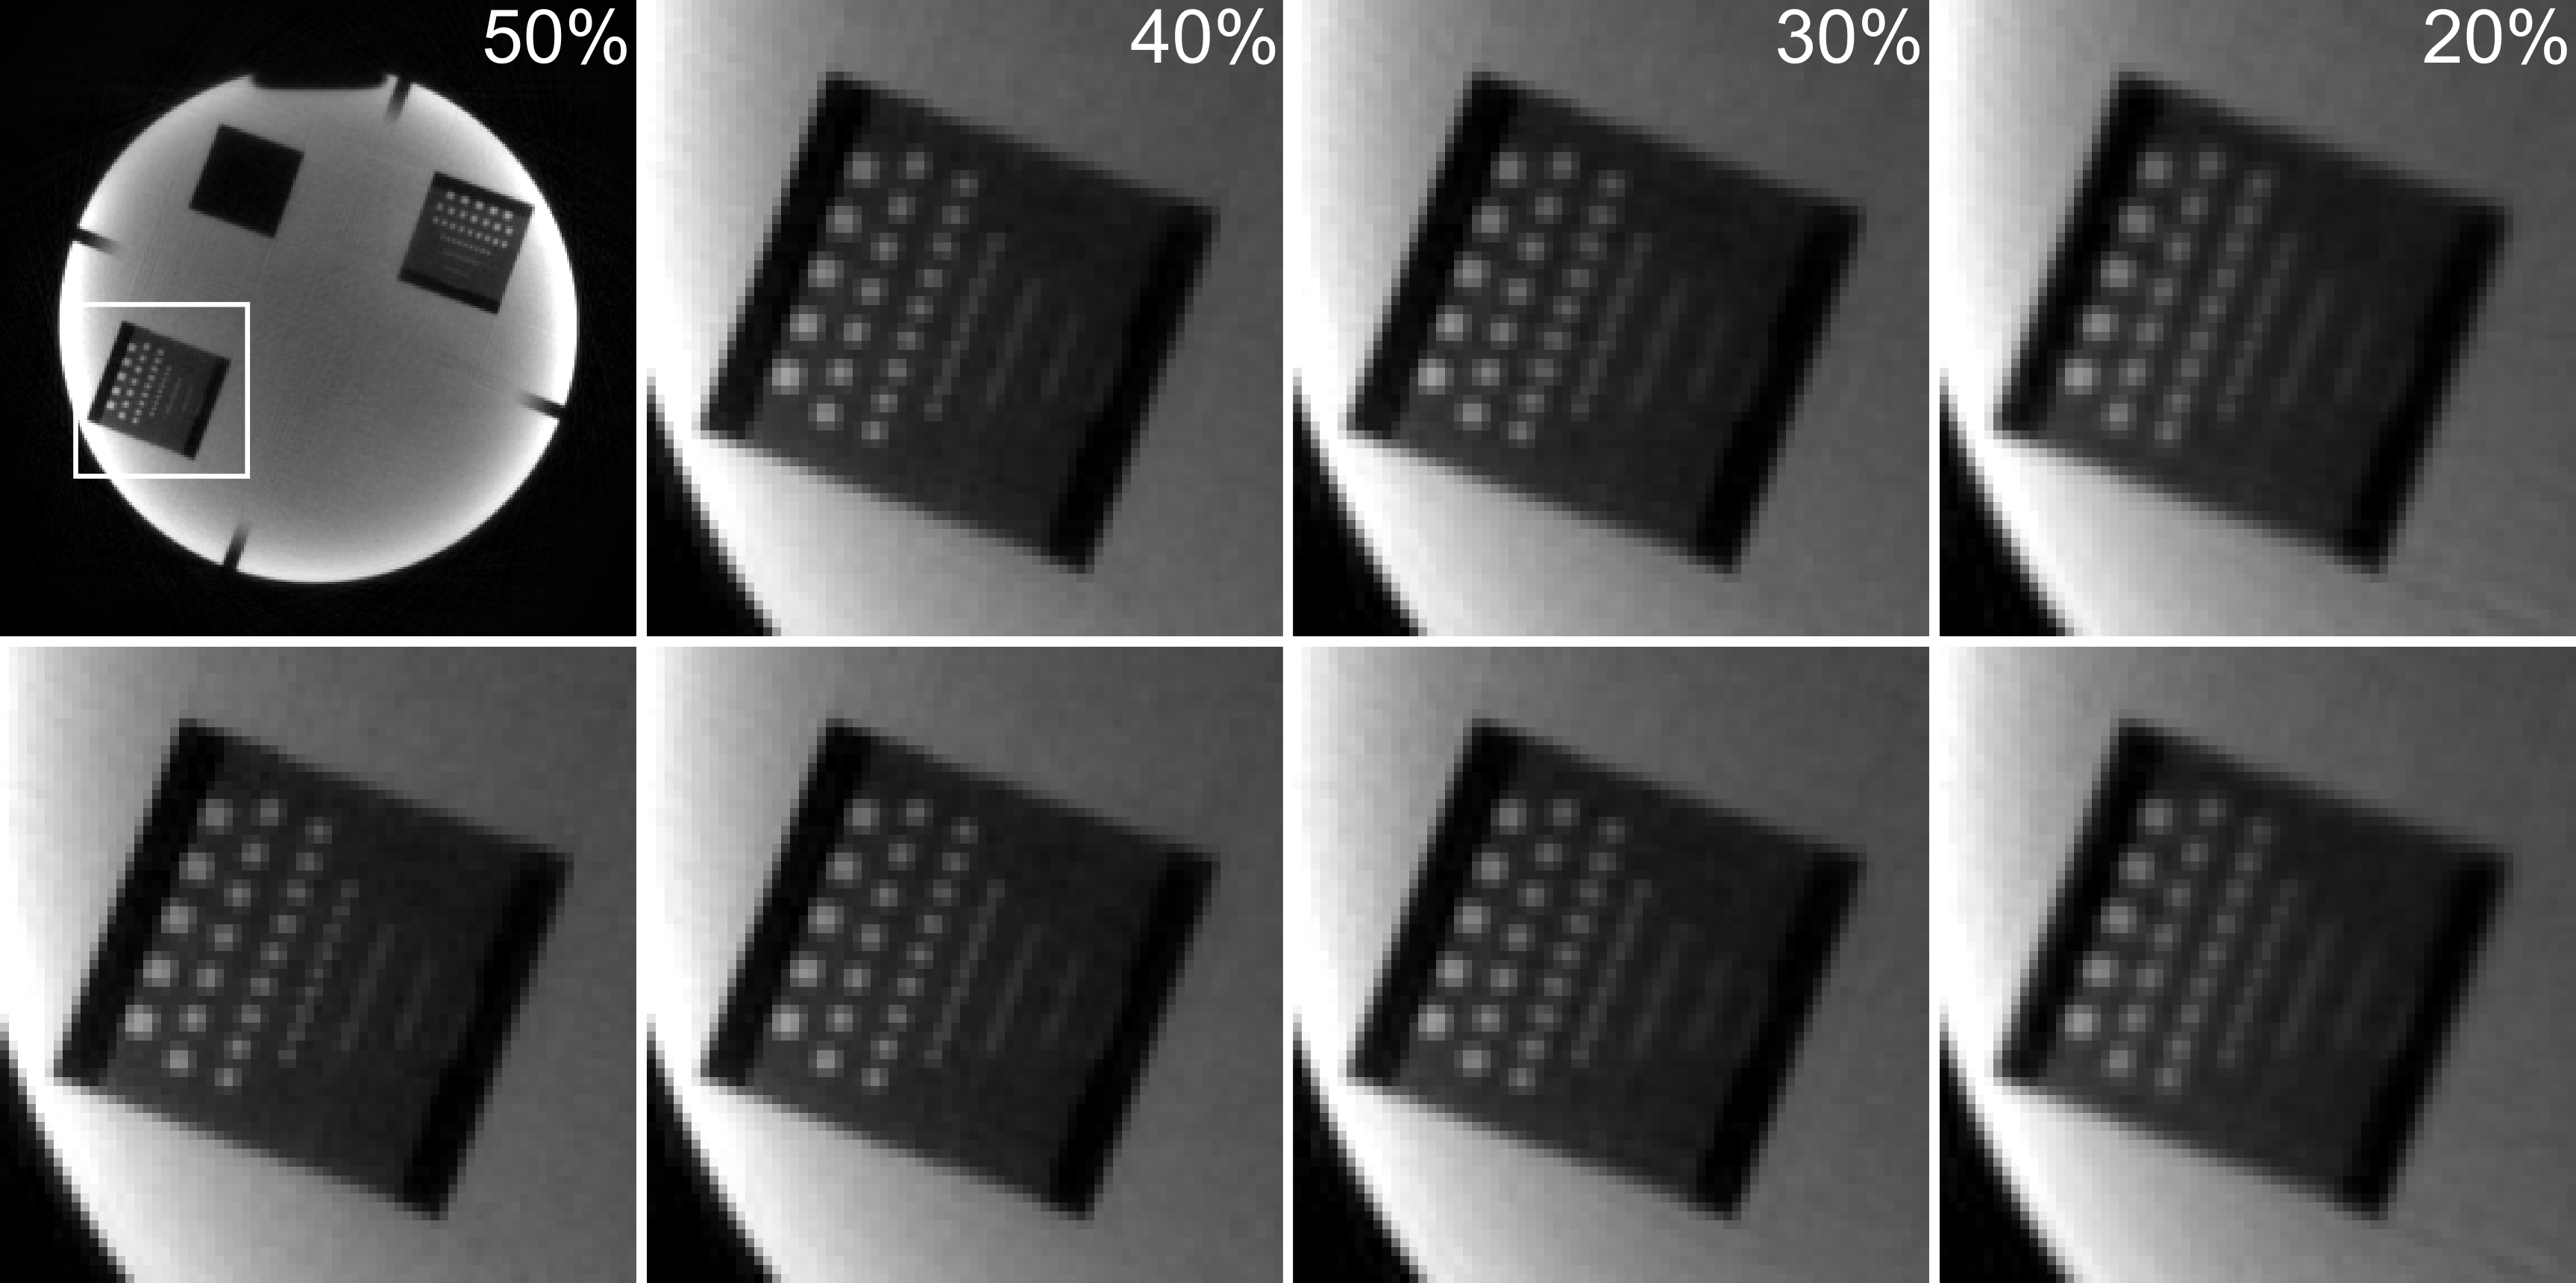
\includegraphics[width=\textwidth]{fig/asym-echo-spatialRes.png}
  \caption{Image reconstructions of a resolution phantom using symmetric gradient echoes (\SI{50}{\percent}) as well as gradient echoes with \SI{40}{\percent}, \SI{30}{\percent}, and \SI{20}{\percent} asymmetry. For asymmetric cases the top panels refer to simulated data obtained by retrospective cropping of data samples of complete spokes, while the bottom panels represent true asymmetric acquisitions with shortest TR and TE. The size of the water-filled holes (and gaps between) in the first three rows are \SI{2.5}{\mm}, \SI{2.0}{\mm}, and \SI{1.5}{\mm} respectively.} \label{Fig:aysm-echo-spatialRes}
\end{figure}

Furthermore, the reduction of TE in asymmetric-echo sampling reduces the sensitivity to off-resonance effect. This property is advantageous in imaging tissues with small $T_2^*$ (e.g.~lung imaging) and slices with strong susceptibilities (e.g.~air-tissue interface). 

\section{Image Reconstructions}
Partial Fourier imaging exploits the conjugate complex symmetry of the full k-space of a real image with zero phase. It is, therefore, widely used to accelerate the acquisition of radiofrequency-refocused spin-echo images. For most gradient-echo images, however, the real-image assumption is violated due to system imperfections and off-resonance contributions from various biological and technical sources, which render the image complex. Previous proposals to deal with complex datasets are synchronous homodyne detection \cite{1991_homodyne}, the projection onto convex sets (\acs{POCS}) method \cite{1991_POCS}, and phase-constrained parallel imaging \cite{2005_PFPPI,2005_phaConstrain_PI}. These approaches assume a certain smoothness of the image phase to justify the calculation of a low-resolution phase map from only the central (i.e. symmetrically covered) k-space region, which is then used to estimate the missing data. More advanced image reconstruction technique, e.g.~NLINV, can directly apply a real-constraint onto the estimated proton density without the pre-calibration of a smooth phase map from the central k-space \cite{2009_Uecker_Thesis}. This real-constrained NLINV, however, totally relies on the conjugate complex symmetry and hence precludes the imaginary part of the estimate proton density, which is insufficient in the cases where phase information is required, e.g., phase-contrast flow imaging and quantitative susceptibility mapping. This study, therefore, exploited the general applicability of NLINV to directly reconstruct complex images and coil sensitivity maps from undersampled asymmetric radial gradient-echo acquisitions.

\section{Application to Real-Time Phase-Contrast Flow MRI}
The implementation of real-time phase-contrast flow MRI is especially challenging because it requires at least two acquisitions with different velocity-encoding gradients that prolong echo times and repetition times. Additional timing problems arise for the incorporation of velocity-compensating gradient waveforms in multiple dimensions. Therefore, this work extends earlier attempts to real-time phase-contrast flow MRI using spiral trajectories \cite{2000_color_flow_MRM,2008_color_flow_MRI} as well as our own recent approaches \cite{2012_PC_Joseph,2014_PC_Joseph} by evaluating the use of asymmetric echoes for radial FLASH sequences with phase-sensitive NLINV reconstruction. The technique advances proposals of asymmetric radial trajectories for ECG-synchronized cine MRI \cite{2014_asym-echo_ISMRM,2014_sTE_flow_ISMRM} to highly undersampled acquisitions suitable for real-time MRI as high temporal resolution. In general, shorter gradient-echo times may be used to reduce the sensitivity to magnetic field inhomogeneities, to acquire more data, to enhance the temporal resolution or to ameliorate the time penalty of motion-compensating gradient waveforms. In short, the purpose of this work was to explore asymmetric radial gradient echoes for real-time phase-contrast flow MRI to allow for velocity compensation in both slice and read directions and thereby reduce the sensitivity of complex blood flow and respective phase errors as commonly observed in patients with cardiovascular disease.

\subsection{Methods}
\cref{Fig:aysm-echo-seq-pc} shows a phase-contrast flow MRI sequence with asymmetric-echo radial FLASH. The sequence diagrams represent two repetitions without and with velocity-encoding gradient, corresponding to the one-sided velocity-encoding scheme. The two TR intervals represent the same spoke from sequential image acquisition (flow-compensated acquisition first and then flow-encoded acquisition, and these two acquisitions encode the same spokes in k-space). The diagrams correctly display the used gradient waveforms (i.e., durations and strengths) for \SI{30}{\percent} asymmetry and VENC = \SI{150}{\cm\per\second} (for other parameters see \cref{Tab:asym-echo-acq}).
\begin{figure}[tb]
  \centering
  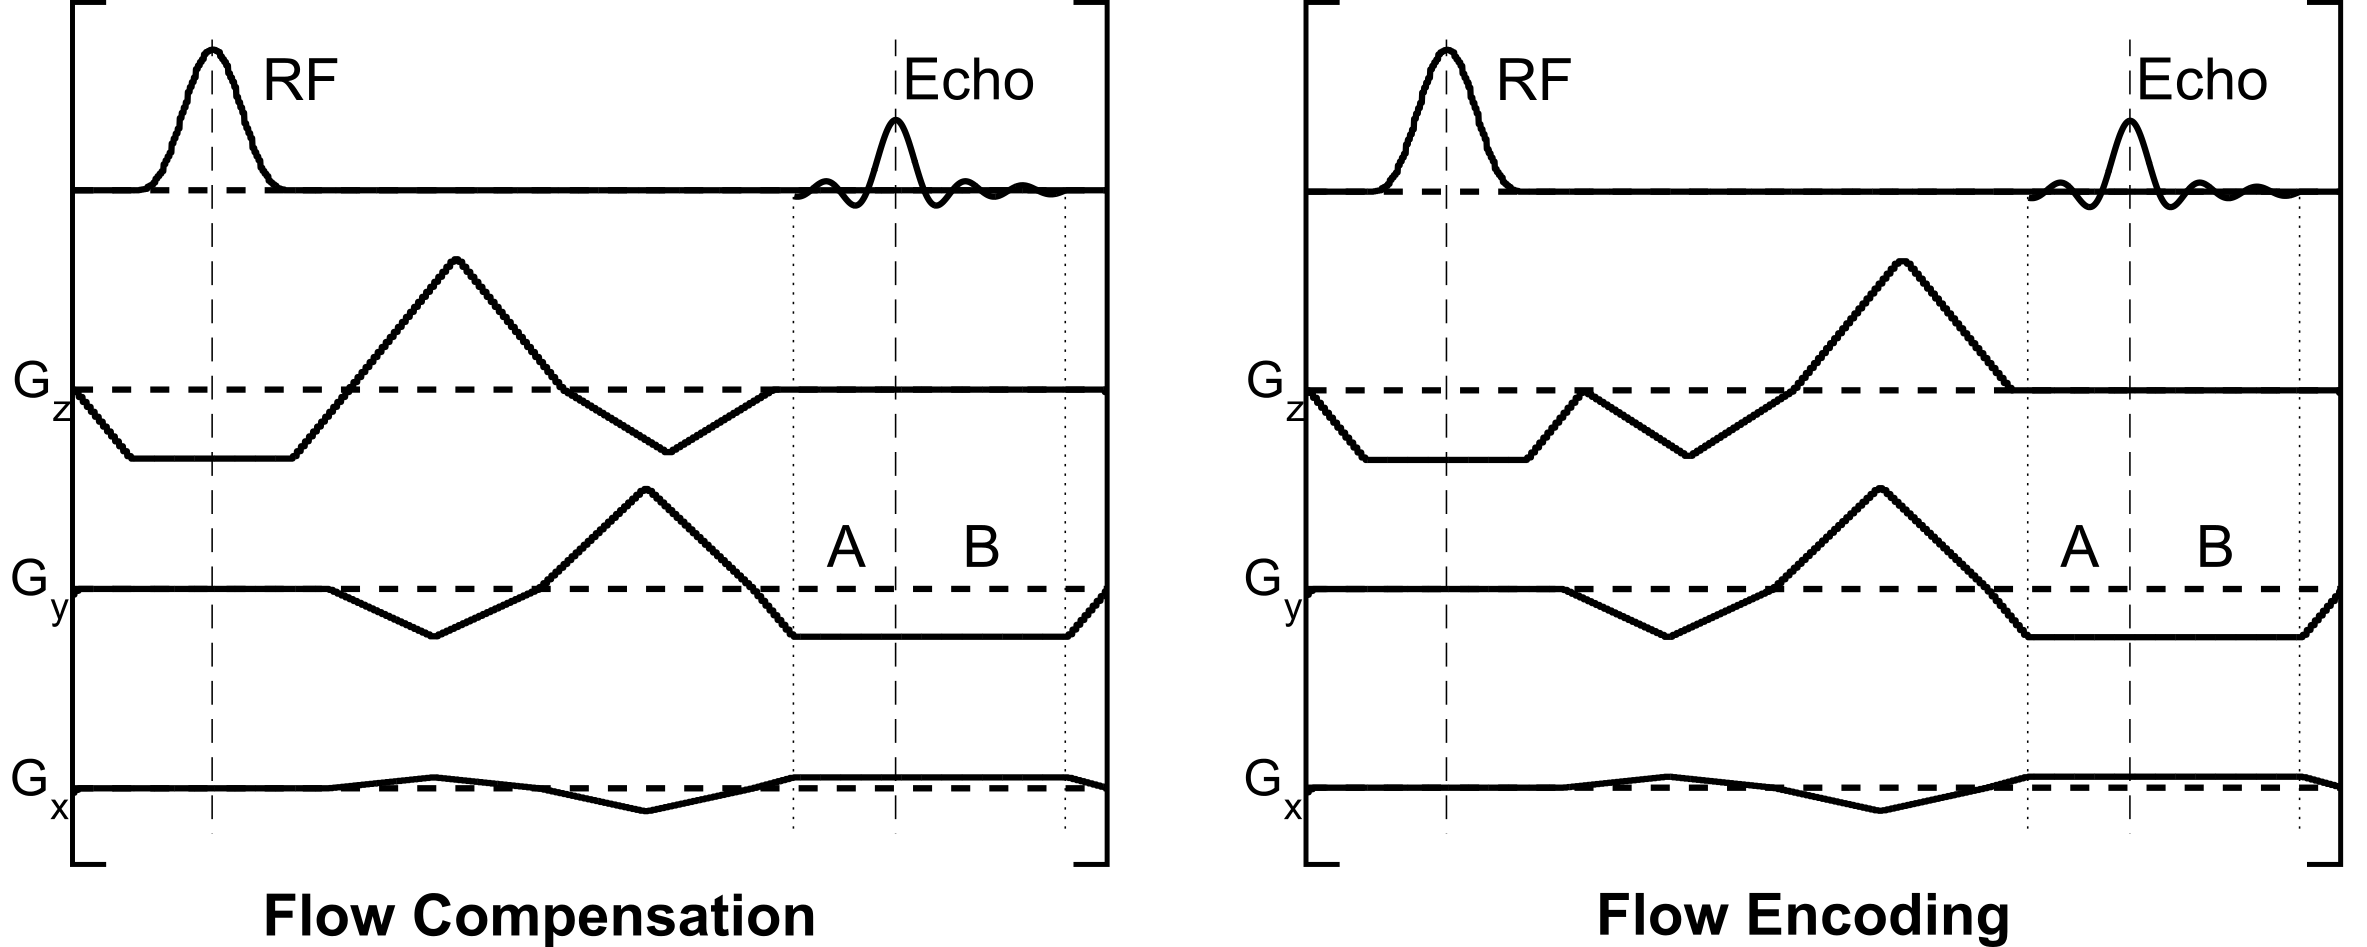
\includegraphics[width=\textwidth]{fig/asym-echo-seq-pc.png}
  \caption{Real-time velocity-encoded radial FLASH with velocity compensation and asymmetric gradient echoes. The sequence diagrams represent corresponding repetition cycles: (Left) Acquisition with velocity-compensated gradients with the waveform $1 \bar{2} 1$ on all axes and overlap the slice selection gradient and the two prephasing read gradients, respectively. (Right) Acquisition with velocity-encoded gradient on the slice selection axis to encode through-plane velocities, and with velocity-compensated gradients on the two read axes to spoil transversal motions.} \label{Fig:aysm-echo-seq-pc}
\end{figure}

\begin{table}[tb]
  \caption{Exemplary acquisition parameters for real-time phase-contrast flow MRI}
  \label{Tab:asym-echo-acq}
  \begin{center}
	\begin{tabular}{ l 
					 c 
					 c 
				   }
	  \toprule
	  Field of view (\si{\square\mm})        & $192 \times 192$        & $320 \times 320$ \\
	  Image matrix size                      & $136 \times 136$        & $212 \times 212$ \\
	  In-plane resolution (\si{\square\mm})  & $1.4 \times 1.4$        & $1.5 \times 1.5$ \\
	  Section thickness (\si{\mm})           & $6$                     & $6$              \\
	  Asymmetry                              & \SI{20}{\percent}     & \SI{30}{\percent} \\
	  Minimum VENC (\si{\cm\per\second})     & $150$                   & $150$               \\
	  Velocity compensation                  & Slice \& $2\times$ Read & Slice \& $2\times$ Read \\
	  Repetition time (\si{\ms})             & 2.38                  & 2.55 \\
	  Echo time (\si{\ms})                   & 1.59                  & 1.70 \\
	  Bandwidth (\si{\hertz\per\pixel})      & 1360                  & 1180 \\
	  Flip angle (\si{\degree})              & 10                    & 10 \\
	  Spokes per frame                       & 7                     & 7 \\
	  Time per frame (\si{\ms})              & 16.66                 & 17.85 \\
	  Time per phase-contrast map (\si{\ms}) & 33.32                 & 35.70 \\
	  Temporal resolution (\si{\fps})        & 30                    & 28 \\
	  \bottomrule
    \end{tabular}
  \end{center}
\end{table}

Five young volunteers without known illness and one patient with combined aortic valve insufficiency and stenosis were recruited for real-time phase-contrast flow evaluations of the ascending aorta. Written informed consent, according to the recommendations of the local ethics committee, was obtained from all subjects before MRI studies, which were performed at \SI{3}{\tesla} using a state-of-the-art MRI system with \SI{80}{\milli\tesla\per\meter} gradients (Magnetom Prisma, Siemens Healthcare, Erlangen, Germany). While phantom studies used the standard \num{64}-channel head coil, human cardiac blood flow was measured by combining an \num{18}-element thorax coil with \num{32} elements of the spine coil. 

For real-time phase-contrast flow MRI with velocity compensation in slice and read directions the outcome of the sequence optimization and reconstruction process led to multiple acquisition protocols. Two relevant examples for a small and large FOV are summarized in \cref{Tab:asym-echo-acq}. In comparison to echo and repetition times of TR/TE = \num{2.86}/\SI{1.93}{\ms} previously reported for symmetric-echo acquisitions without in-plane velocity compensation and a measuring time of \SI{40}{\ms} \cite{2014_PC_Joseph}, the current values of TR/TE = \num{2.38}/\SI{1.59}{\ms} (FOV = \SI{192}{\mm}) and TR/TE = \num{2.55}/\SI{1.70}{\ms} (FOV = \SI{320}{\mm}) offer even faster acquisitions with total measuring times of \SI{33.3}{\ms} and \SI{35.7}{\ms}, respectively. While these numbers refer to a minimum VENC of \SI{150}{\cm\per\second}, the latter implementation would be prolonged to \SI{40}{\ms} when using \SI{75}{\cm\per\second}.

Blood flow was measured in the ascending aorta at the level of the right pulmonary artery. Typically, real-time flow MRI acquisitions of human subjects were performed during free breathing at \SI{35.7}{\ms} resolution and for a period of \SI{12.5}{\second} yielding \num{350} magnitude images and phase-contrast maps. For comparison, free-breathing ECG-synchronized cine phase-contrast flow MRI with Cartesian encoding and retrospective sorting (standard sequence of the vendor) was performed at \SI{1.54 x 1.54}{\mm} in-plane resolution and \SI{6}{\mm} section thickness. This conventional technique also used velocity compensation for all imaging gradients. Other experimental parameters: TR = \SI{20.00}{\ms}, TE = \SI{2.73}{\ms}, flip angle = \ang{20}, \num{3} averages, \num{30} cardiac phases, FOV = \SI{220 x 320}{\square\mm}, matrix resolution \num{144x208}.

Before NLINV reconstruction, the datasets from multiple coils are first corrected for gradient delay errors \cite{2015_PC_Asym} and then compressed to \num{10} virtual channels with coefficients calculated by principal component analysis to reduce the amount of computational load for image reconstruction. After NLINV, quantitative analyses of phase-contrast flow MRI images and evaluations of respective flow parameters were obtained with the use of CAIPI prototype software (Franhofer MEVIS, Bremen, Germany), especially modified for the automated analysis of real-time MRI acquisitions (typically \num{10} cardiac cycles).


\subsection{Results}
\subsubsection*{Phantom Studies}
\cref{Fig:aysm-echo-pha} summarizes the results of a real-time phase-contrast flow MRI study of a phantom where the left and right panels refer to perpendicular image orientations. All magnitude images and corresponding phase-contrast maps represent selected single frames from real-time phase-contrast flow MRI movies at \SI{33.3}{\ms} resolution with velocity compensation (top) in slice direction and (bottom) in slice and read directions (experimental details in \cref{Tab:asym-echo-acq}). The rapid water flow in the inner tubing (in reverse direction to slower flow in the outer tubing) is characterized by turbulence. With velocity compensation in slice direction only and symmetric echo acquisitions the magnitude images suffer from substantial signal void due to extensive intravoxel phase dispersion, while the corresponding phase-contrast maps exhibit multiple phase wraps due to unwanted phase contributions from in-plane flow components. In contrast, the velocity-compensated flow MRI acquisitions in all directions with \SI{20}{\percent} asymmetry, result in magnitude images with fully recovered signal intensities, while the phase-contrast maps are no longer contaminated by phase wraps, but instead reveal phase values that exclusively represent the desired through-plane flow components. This is particularly well seen in the lower-right phase-contrast map where the flow direction in the arch of the inner tube changes its direction by \ang{180} (i.e., from dark to bright intensities).

\subsubsection*{Human Studies}
To assess the robustness and accuracy of the real-time flow MRI technique with full velocity compensation, \cref{Tab:asym-echo-quant} summarizes the result of a study of five healthy subjects and a patient with combined aortic valve insufficiency and stenosis. These data were acquired with experimental parameters as given for the \SI{320}{\mm} FOV in \cref{Tab:asym-echo-acq}. The quantitative evaluations in \cref{Tab:asym-echo-quant} compare peak flow velocities, flow per heartbeat, flow volumes and regurgitation fractions for real-time flow MRI with velocity compensation in the slice direction only, with velocity compensation in slice and read directions and conventional ECG-synchronized cine flow MRI with velocity compensation. The results for real-time MRI represent mean values $\pm$ standard deviation for \num{10} consecutive heartbeats.

For the patient a meaningful evaluation of the real-time flow MRI data without in-plane velocity compensation was impossible because of significant turbulence. In close analogy to the phantom results shown in \cref{Fig:aysm-echo-pha}, the poor performance of the old method and the corrected behavior of the proposed method are demonstrated in \cref{Fig:aysm-echo-pat}. The left and right panels refer to two positions along the aorta, i.e., at the level of the pulmonary artery and close to the aortic valve, respectively. With velocity compensation in slice direction only, the magnitude images exhibit a complete signal void in the aorta, while the corresponding phase-contrast maps suffer from multiple phase wraps. In contrast, the magnitude images from fully compensated acquisitions with \SI{30}{\percent} asymmetry maintain the full (inflow) MRI signal and in the phase-contrast maps re-establish phase profiles that represent the true through-plane velocities without phase wraps. These velocity profiles are pathologically distorted compared with the observation of almost laminar flow with parabolic velocity distribution in healthy subjects, e.g. see Joseph et al.~\cite{2012_PC_Joseph}.

\begin{figure}[p]
  \centering
  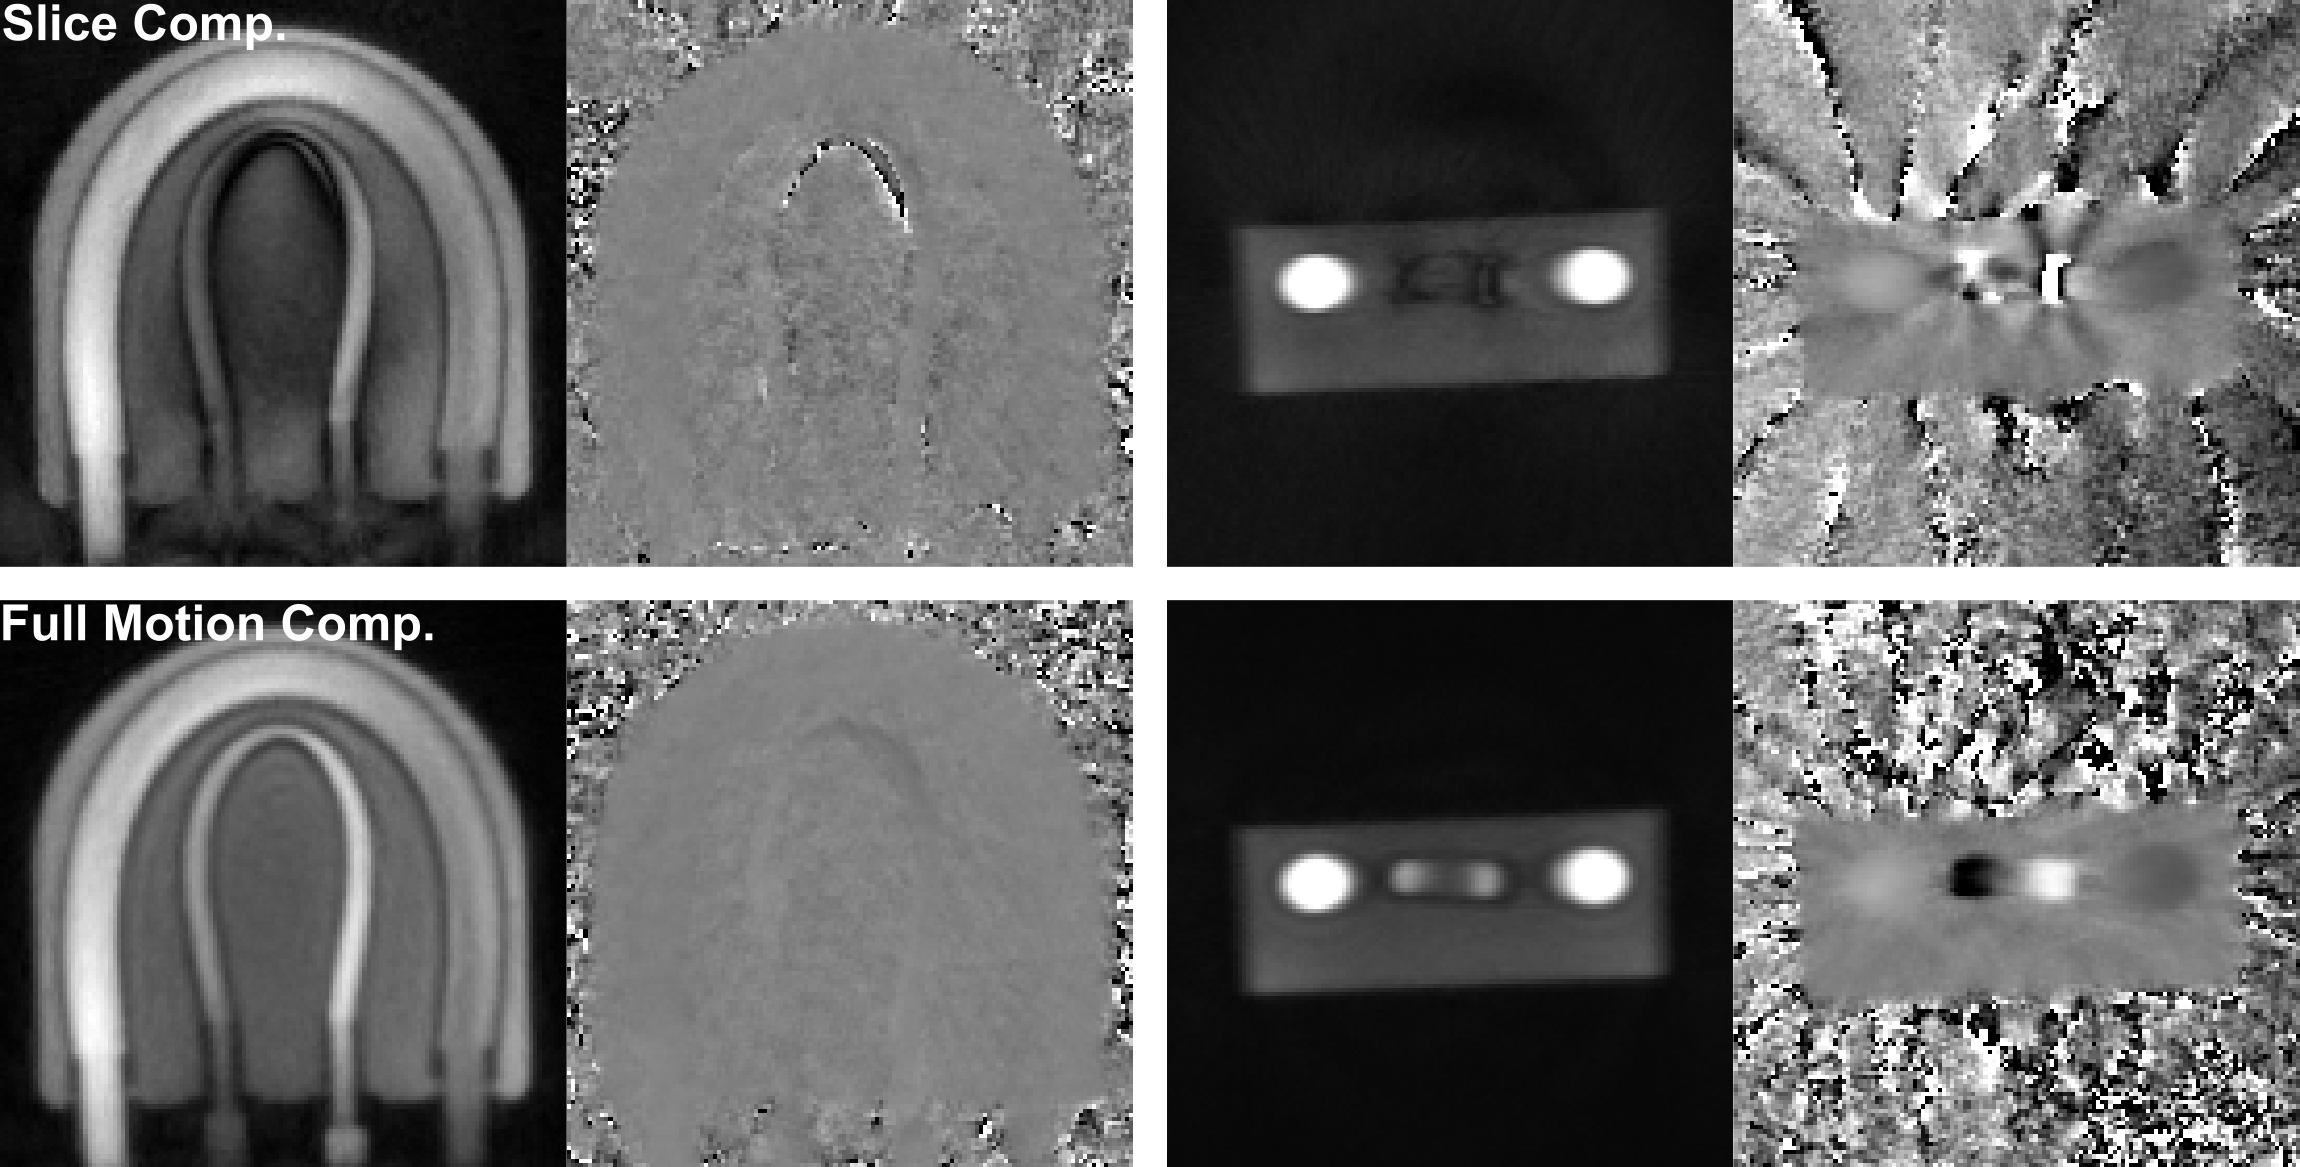
\includegraphics[width=0.80\textwidth]{fig/asym-echo-pha.png}
  \caption{Real-time phase-contrast MRI (\SI{33.3}{\ms} temporal resolution, FOV = \SI{192}{\mm}) of through-plane flow in a phantom with complex flow in the inner small tube. The panels represent selected magnitude images and corresponding phase-contrast maps in a coronal (left) and transverse (right) view at the arch of the inner tube. The images were obtained with velocity-compensating gradient waveforms (top) in slice direction only using symmetric radial gradient echoes and (bottom) in slice and read directions using gradient echoes with \SI{20}{\percent} asymmetry.} \label{Fig:aysm-echo-pha}
  
  \par\bigskip
  
  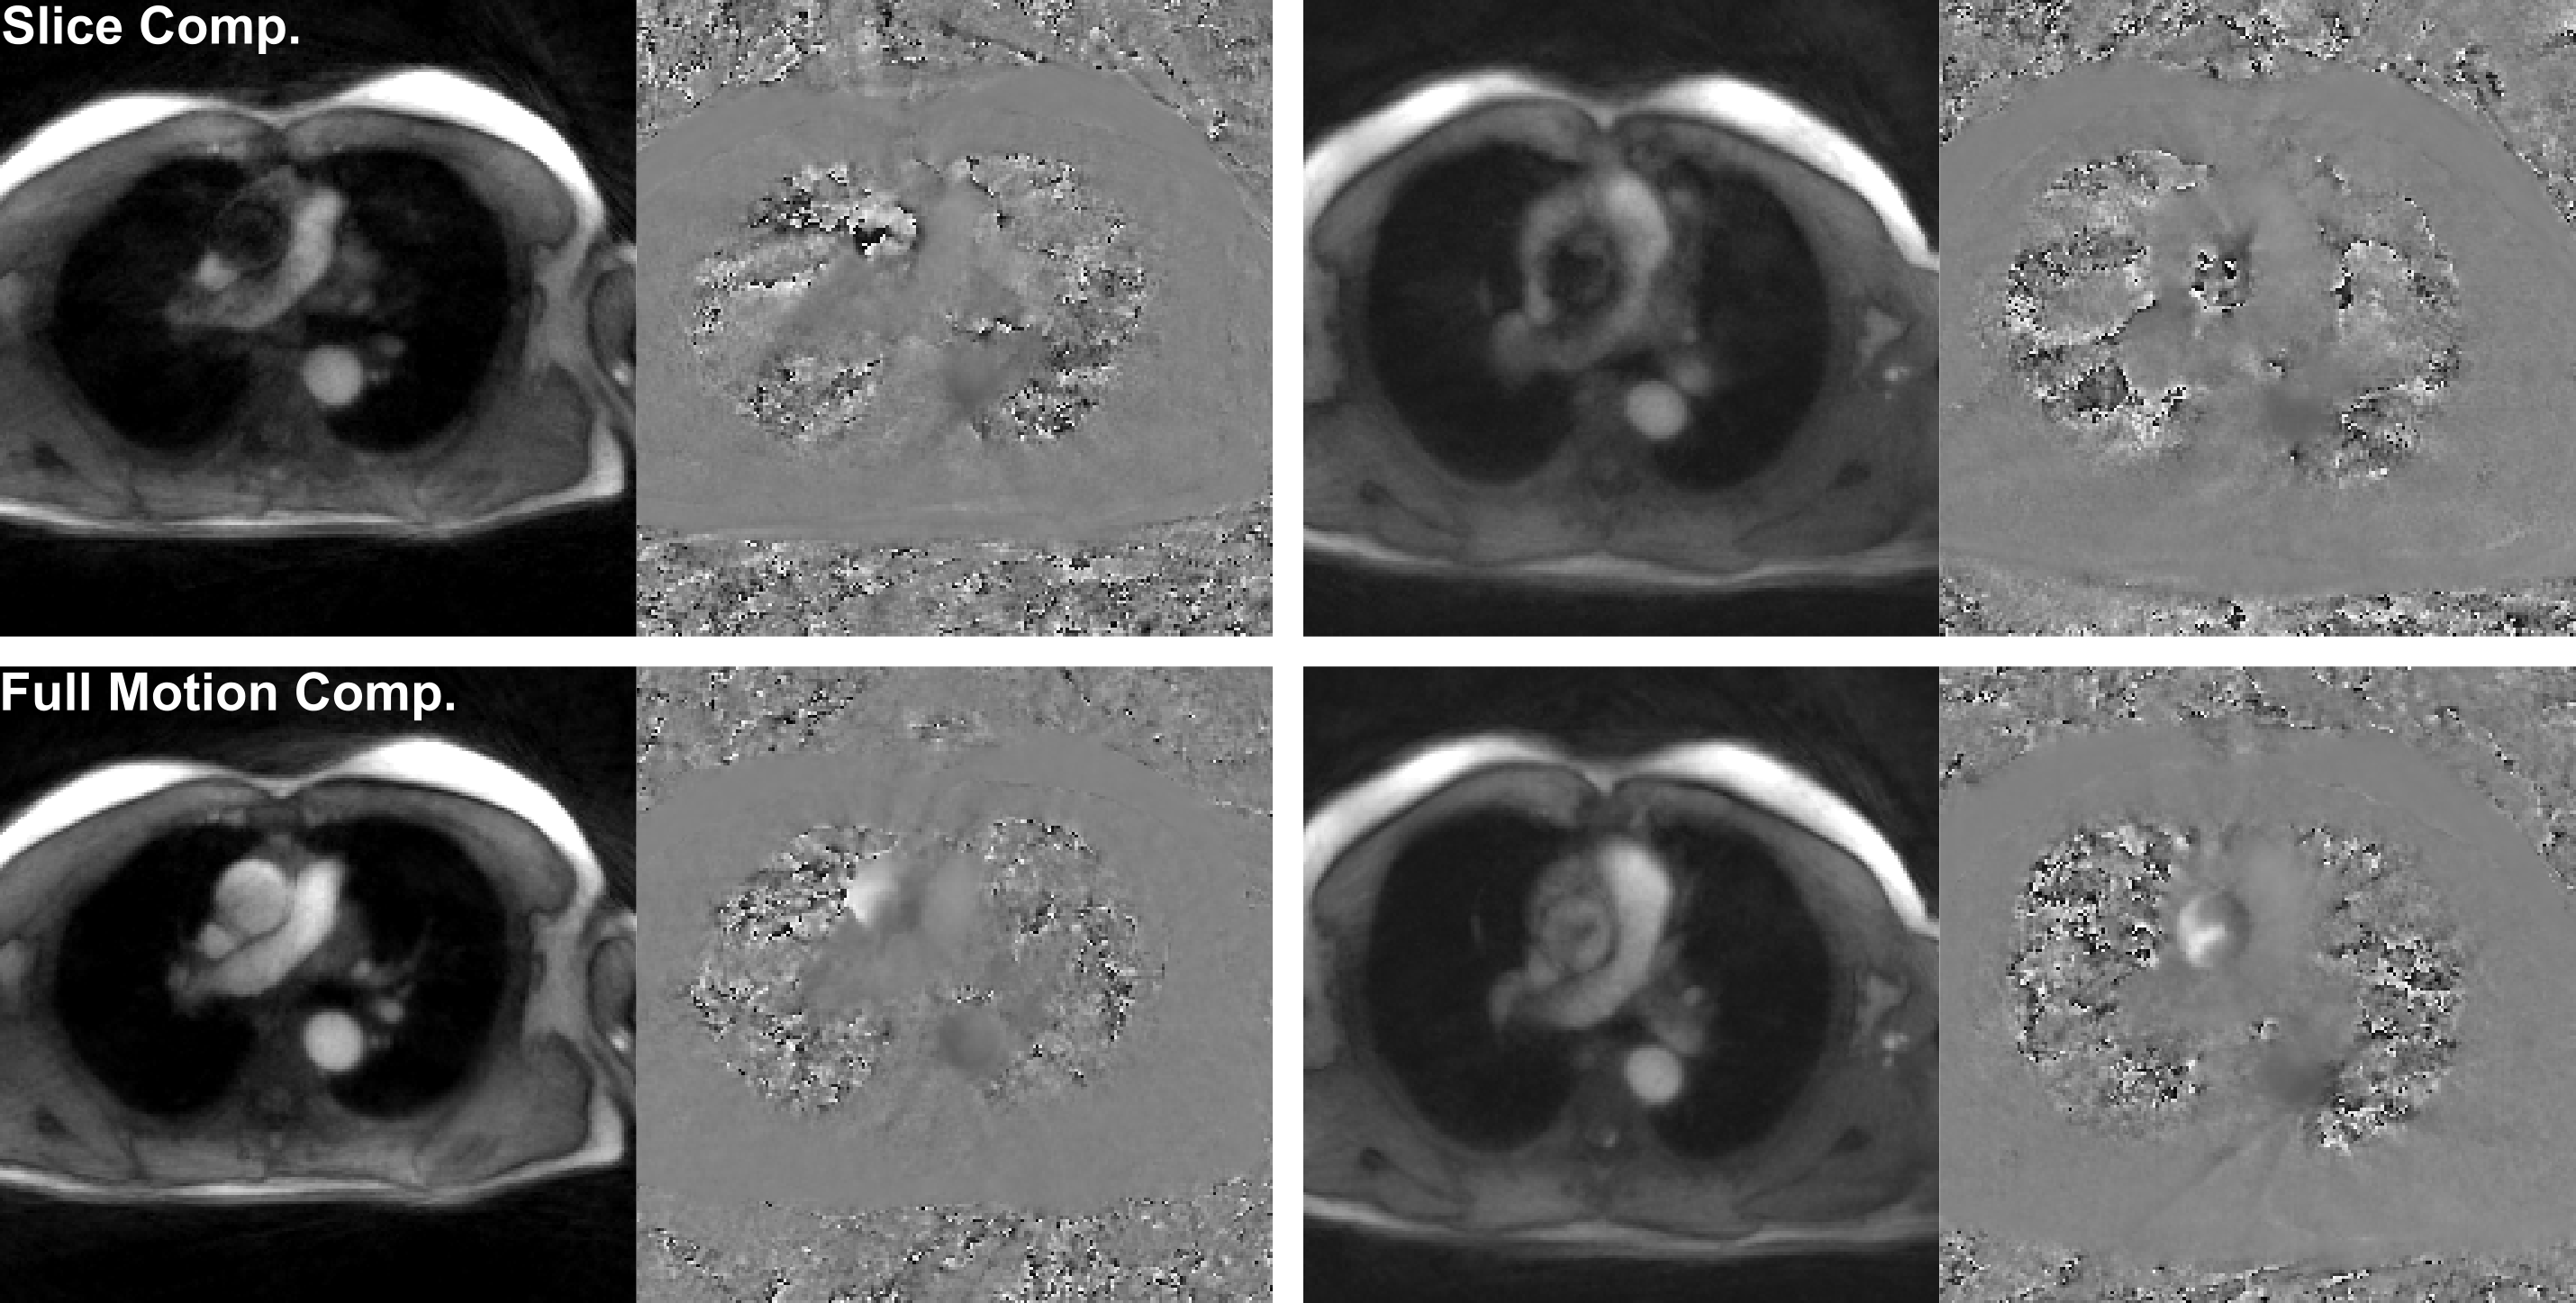
\includegraphics[width=0.80\textwidth]{fig/asym-echo-pat.png}
  \caption{Real-time phase-contrast MRI of aortic blood flow (\SI{35.7}{\ms} temporal resolution, FOV = \SI{320}{\mm}) for a patient with combined aortic valve insufficiency and stenosis. The panels represent selected magnitude images and corresponding phase-contrast maps of the ascending aorta at the level of the pulmonary artery (left) and close to the aortic valve (right). The images were obtained with velocity-compensating gradient waveforms in slice direction only using symmetric radial gradient echoes (top) and in slice and read directions using gradient echoes with \SI{30}{\percent} asymmetry (bottom).} \label{Fig:aysm-echo-pat}
\end{figure}

\begin{table}[tb]
  \caption{Quantitative flow evaluations in the ascending aorta of healthy volunteers and a patient with valve insufficiency\textsuperscript{1}}
  \label{Tab:asym-echo-quant}
  \begin{center}
    \begin{threeparttable}
      \begin{tabular}{ 	c 
                        c 
					    S[table-format=3(2)]
					    S[table-format=3(2)]
					    S[table-format=1.1(2)]
					    S[table-format=2(1)] 
				     }
        \toprule
        \multirow{2}{*}{Subject} & \multirow{2}{*}{MRI} & {Peak Velocity}         & {Flow per}                  & {Flow Volume}          & {Regurgitation}            \\
                                 &                      & {(\si{\cm\per\second})} & {Heartbeat (\si{\milli\L})} & {(\si{\L\per\minute})} & {Fraction (\si{\percent})} \\
		\midrule
        \multirow{3}{*}{No.1}    & {RT-Slice\textsuperscript{2}} & 132\pm7  &  91\pm4 & 5.5\pm0.2 & 2\pm1  \\
                                 & {RT-All\textsuperscript{3}}   & 120\pm3  &  95\pm6 & 5.4\pm0.4 & 2\pm1  \\
                                 & {Cine}                        & 140      & 116     & 7.1       & 1      \\
        \hline
	    \multirow{3}{*}{No.2}    & {RT-Slice}                    & 129\pm9  & 131\pm6 & 7.7\pm0.5 & 1\pm1  \\
	                             & {RT-All}                      & 112\pm9  & 123\pm6 & 6.9\pm0.3 & 1\pm1  \\
	                             & {Cine}                        & 126      & 133     & 7.9       & 1      \\
	    \hline
	    \multirow{3}{*}{No.3}    & {RT-Slice}                    &  76\pm4  &  57\pm4 & 4.0\pm0.2 & 2\pm1  \\
                                 & {RT-All}                      &  69\pm4  &  55\pm1 & 3.6\pm0.2 & 2\pm1  \\
                                 & {Cine}                        &  76      &  65     & 4.3       & 1      \\
	    \hline
	    \multirow{3}{*}{No.4}    & {RT-Slice}                    & 122\pm19 & 126\pm10 & 8.9\pm3.1 & 2\pm1  \\
                                 & {RT-All}                      & 113\pm6  & 121\pm3  & 7.5\pm0.2 & 2\pm1  \\
                                 & {Cine}                        & 117      & 111      & 7.4       & 2      \\
        \hline
   	    \multirow{3}{*}{No.5}    & {RT-Slice}                    & 120\pm8  &  89\pm2  & 5.1\pm0.2 & 5\pm1  \\
                                 & {RT-All}                      & 100\pm6  &  91\pm4  & 5.3\pm0.2 & 5\pm1  \\
                                 & {Cine}                        & 107      & 102      & 6.1       & 4      \\
		\hline
   	    \multirow{2}{*}{Patient} & {RT-All}                      & 260\pm15 &  49\pm7  & 2.7\pm0.5 & 58\pm5  \\
                                 & {Cine}                        & 253      &  50      & 2.6       & 64      \\
	    \bottomrule
      \end{tabular}
  
      \begin{tablenotes}
	    \small
	    \item[1] Results represent mean values $\pm$ standard deviation for \num{10} consecutive heartbeats.
	    \item[2] RT-Slice, real-time flow MRI with velocity compensation in slice direction only.
	    \item[3] RT-All, real-time flow MRI with velocity compensation in slice and read directions.
	  \end{tablenotes}
    \end{threeparttable}
  \end{center}
\end{table}



\subsection{Discussion}
The proposed method for reconstructing highly undersampled asymmetric radial MRI data relies on NLINV \cite{2008_NLINV,2010_NLINV_Heart,2010_20ms_Uecker} with a suitable gradient delay correction. The results obtained for a resolution phantom not only confirm the reliability of the estimated gradient delays for highly undersampled asymmetric echoes, but also demonstrate the achievable image quality and spatial resolution. Only for \SI{20}{\percent} asymmetry the row of \SI{1.5}{\mm} holes in \cref{Fig:aysm-echo-spatialRes} exhibits a slight blurring. This phenomenon reflects the relatively higher fraction of low k-space values in an asymmetric versus a symmetric radial dataset, which for a given weight of the NLINV regularization yields a corresponding overestimation of low spatial frequencies. In principle, the effect may, therefore, be reduced by decreasing the regularization weight which may be accomplished by increasing the number of iterative Gauss-Newton steps used for NLINV reconstruction.

In human studies, complex flow in the ascending aorta with respective multi-dimensional phase contributions is a frequent phenomenon in patients with cardiovascular disease, but not in healthy subjects \cite{2012_PC_Joseph,2014_PC_Joseph}. Nevertheless, a comparison of real-time acquisitions without and with compensation of in-plane phase components reveals approximately \num{10}-\SI{20}{\percent} lower peak flow velocities for later method (see \cref{Tab:asym-echo-quant}). Because velocities directly represent phase information, this observation indicates the successful removal of some false positive phase contributions by the proposed method even in healthy volunteers. In the absence of a gold standard a comparison of these results with those obtained by cine flow MRI are less instructive in view of phase information in real-time acquisitions and the combination of phase information for multiple cardiac cycles in a cine acquisition. However, despite these problems, the flow results obtained for the proposed real-time flow MRI method and the conventional cine MRI method are in general agreement including values for the patient with aortic valve dysfunction.

In conclusion, the development of asymmetric echoes for highly undersampled radial FLASH sequences offers significant technical advances for real-time phase-contrast flow MRI, where the incorporation of velocity compensation in slice and read directions without compromising temporal resolution sets the basis for quantitatively accurate studies. The proposed method now warrants further clinical validation and extensive applications.

\section{Summary}
Asymmetric radial gradient echo sampling has been successfully implemented on the MRI scanner, and the simulated and experimental results reveal a usable degree of up to \SI{20}{\percent} asymmetry. The application of asymmetric echo to real-time phase-contrast flow MRI enables the addition of velocity-compensated gradients without contaminating the temporal resolution. Short echo time and velocity compensation are beneficial in flow velocity measurements as they can decrease phase dispersion and spoil accelerated spins. In addition, asymmetric echo sampling with or without motion compensation can be potentially applied to other applications, i.e., speech studies and cardiac imaging, for the gain of acquisition speed. However, the image reconstruction for asymmetric-echo sampled data is limited to the phase-sensitive NLINV method. The integration of advanced phase constraints into NLINV for extreme asymmetric echo (e.g.~asymmetry $<$ \SI{20}{\percent}) could further reduce echo time, probably recover the missing portion of the asymmetric echo, and eventually improve temporal resolutions of real-time MRI. To implement phase-constrained methods, an appropriate regularization on the phase is most likely required, but the extraction of the phase information from the MR signal model in parallel imaging is complicated and thus requires better mathematical treatments in IRGNM.


